\documentclass[twoside]{article}

% Packages required by doxygen
\usepackage{fixltx2e}
\usepackage{calc}
\usepackage{doxygen}
\usepackage[export]{adjustbox} % also loads graphicx
\usepackage{graphicx}
\usepackage[utf8]{inputenc}
\usepackage{makeidx}
\usepackage{multicol}
\usepackage{multirow}
\PassOptionsToPackage{warn}{textcomp}
\usepackage{textcomp}
\usepackage[nointegrals]{wasysym}
\usepackage[table]{xcolor}

% NLS support packages
\usepackage[T2A]{fontenc}
\usepackage[ukrainian]{babel}

% Font selection
\usepackage[T1]{fontenc}
\usepackage[scaled=.90]{helvet}
\usepackage{courier}
\usepackage{amssymb}
\usepackage{sectsty}
\renewcommand{\familydefault}{\sfdefault}
\allsectionsfont{%
  \fontseries{bc}\selectfont%
  \color{darkgray}%
}
\renewcommand{\DoxyLabelFont}{%
  \fontseries{bc}\selectfont%
  \color{darkgray}%
}
\newcommand{\+}{\discretionary{\mbox{\scriptsize$\hookleftarrow$}}{}{}}

% Page & text layout
\usepackage{geometry}
\geometry{%
  a4paper,%
  top=2.5cm,%
  bottom=2.5cm,%
  left=2.5cm,%
  right=2.5cm%
}
\tolerance=750
\hfuzz=15pt
\hbadness=750
\setlength{\emergencystretch}{15pt}
\setlength{\parindent}{0cm}
\setlength{\parskip}{3ex plus 2ex minus 2ex}
\makeatletter
\renewcommand{\paragraph}{%
  \@startsection{paragraph}{4}{0ex}{-1.0ex}{1.0ex}{%
    \normalfont\normalsize\bfseries\SS@parafont%
  }%
}
\renewcommand{\subparagraph}{%
  \@startsection{subparagraph}{5}{0ex}{-1.0ex}{1.0ex}{%
    \normalfont\normalsize\bfseries\SS@subparafont%
  }%
}
\makeatother

% Headers & footers
\usepackage{fancyhdr}
\pagestyle{fancyplain}
\fancyhead[LE]{\fancyplain{}{\bfseries\thepage}}
\fancyhead[CE]{\fancyplain{}{}}
\fancyhead[RE]{\fancyplain{}{\bfseries\leftmark}}
\fancyhead[LO]{\fancyplain{}{\bfseries\rightmark}}
\fancyhead[CO]{\fancyplain{}{}}
\fancyhead[RO]{\fancyplain{}{\bfseries\thepage}}
\fancyfoot[LE]{\fancyplain{}{}}
\fancyfoot[CE]{\fancyplain{}{}}
\fancyfoot[RE]{\fancyplain{}{\bfseries\scriptsize Створено системою Doxygen }}
\fancyfoot[LO]{\fancyplain{}{\bfseries\scriptsize Створено системою Doxygen }}
\fancyfoot[CO]{\fancyplain{}{}}
\fancyfoot[RO]{\fancyplain{}{}}
\renewcommand{\footrulewidth}{0.4pt}
\renewcommand{\sectionmark}[1]{%
  \markright{\thesection\ #1}%
}

% Indices & bibliography
\usepackage{natbib}
\usepackage[titles]{tocloft}
\setcounter{tocdepth}{3}
\setcounter{secnumdepth}{5}
\makeindex

% Hyperlinks (required, but should be loaded last)
\usepackage{ifpdf}
\ifpdf
  \usepackage[pdftex,pagebackref=true]{hyperref}
\else
  \usepackage[ps2pdf,pagebackref=true]{hyperref}
\fi
\hypersetup{%
  colorlinks=true,%
  linkcolor=blue,%
  citecolor=blue,%
  unicode%
}

% Custom commands
\newcommand{\clearemptydoublepage}{%
  \newpage{\pagestyle{empty}\cleardoublepage}%
}

\usepackage{caption}
\captionsetup{labelsep=space,justification=centering,font={bf},singlelinecheck=off,skip=4pt,position=top}

%===== C O N T E N T S =====

\begin{document}

% Titlepage & ToC
\hypersetup{pageanchor=false,
             bookmarksnumbered=true,
             pdfencoding=unicode
            }
\pagenumbering{alph}
\begin{titlepage}
\vspace*{7cm}
\begin{center}%
{\Large Лаборатрна робота 1 }\\
\vspace*{1cm}
{\large Створено системою Doxygen 1.8.14}\\
\end{center}
\end{titlepage}
\pagenumbering{roman}
\tableofcontents
\pagenumbering{arabic}
\hypersetup{pageanchor=true}

%--- Begin generated contents ---
\section{Звіт з лабораторної роботи 1}
\label{index}\hypertarget{index}{}за дисципліною \char`\"{}\+Big Data Application and Analytics\char`\"{} ~\newline
 студента групи ПК-\/21m-\/1 ~\newline
 Панасенка Єгора Сергійовича ~\newline
 Кафедра комп\textquotesingle{}ютерних технологій ~\newline
 ФПМ, ДНУ, 2021-\/2022 навч.\+р. ~\newline
 Варіант 13

Звіт доступний за посиланням ~\newline
 \href{https://gaurapanasenko.github.io/unilab_opt/BDAnA_Labs/html/index.html}{\texttt{ https\+://gaurapanasenko.\+github.\+io/unilab\+\_\+opt/\+BDAn\+A\+\_\+\+Labs/html/index.\+html}}. ~\newline
 Вихідний код доступний за посиланням ~\newline
 \href{https://github.com/gaurapanasenko/unilab/tree/master/09/BDAnA_Labs}{\texttt{ https\+://github.\+com/gaurapanasenko/unilab/tree/master/09/\+BDAn\+A\+\_\+\+Labs}}\hypertarget{index_autotoc_md0}{}\doxysubsection{Постановка задачі}\label{index_autotoc_md0}
 
\begin{DoxyImageNoCaption}
  \mbox{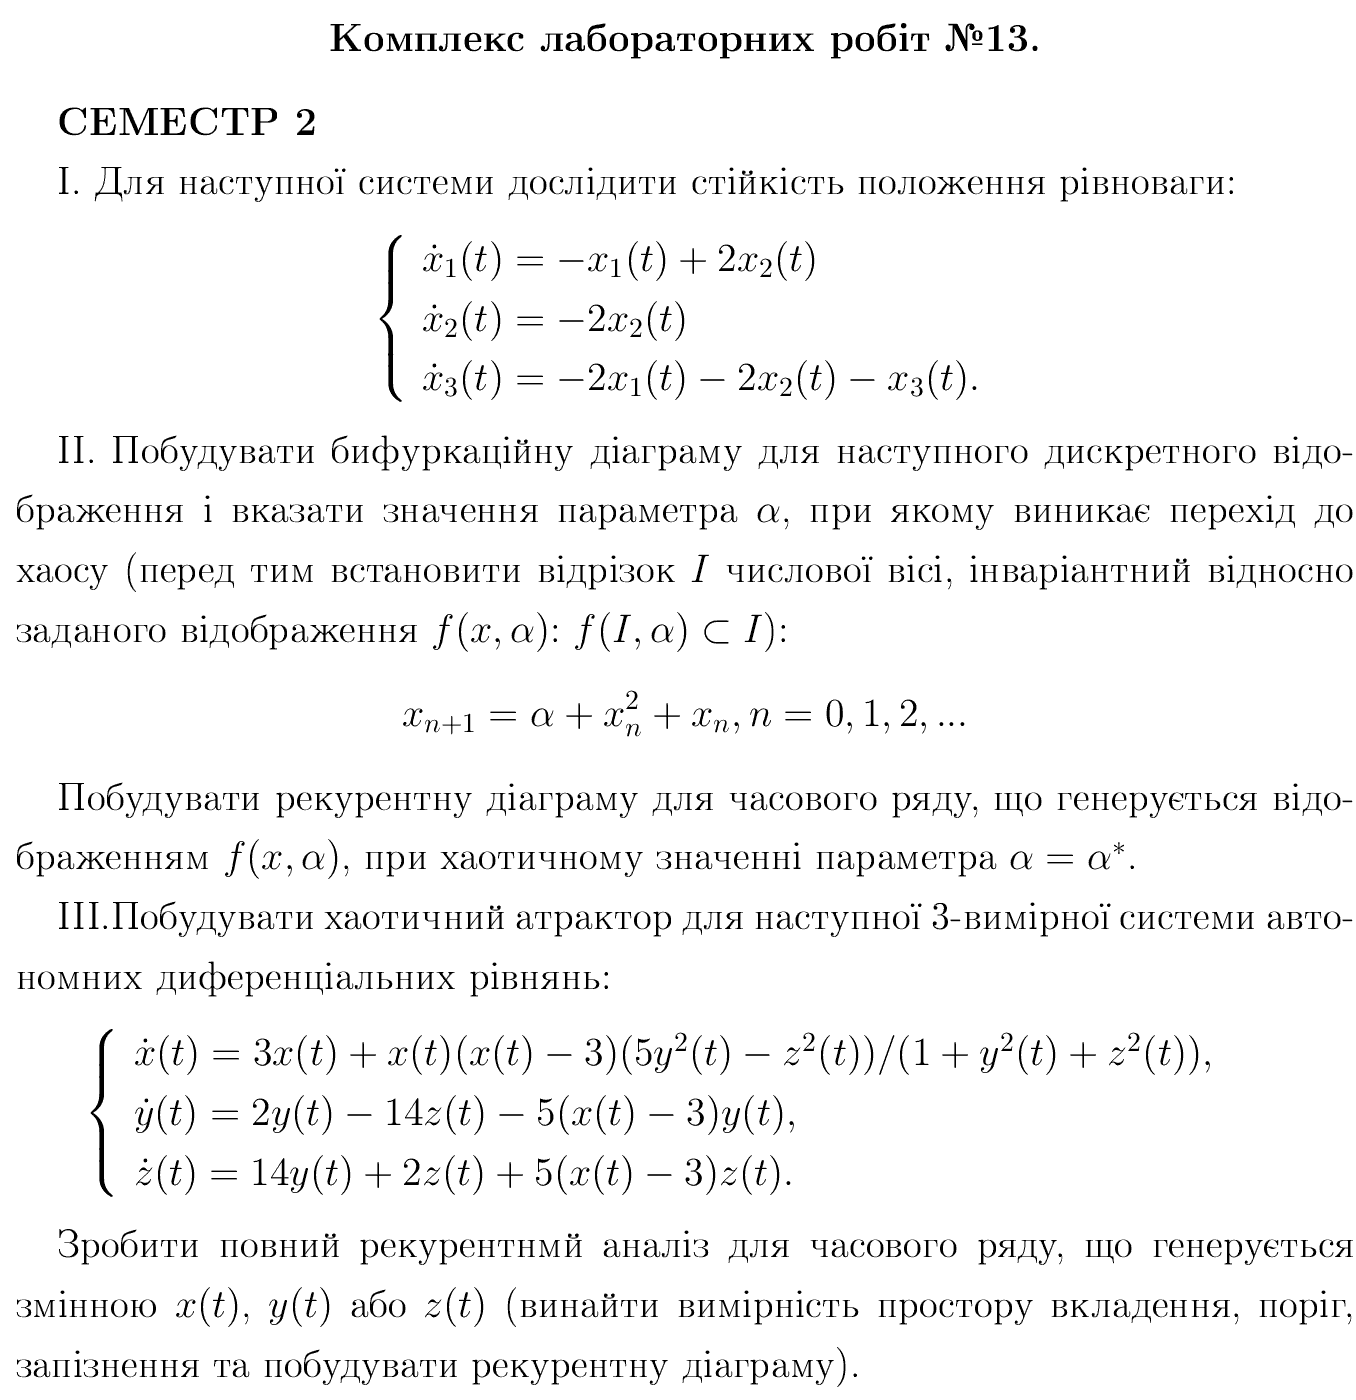
\includegraphics[width=\textwidth,height=\textheight/2,keepaspectratio=true]{Task.png}}
\end{DoxyImageNoCaption}
\hypertarget{index_autotoc_md1}{}\doxysubsection{Отримані результати}\label{index_autotoc_md1}
\hypertarget{index_autotoc_md2}{}\doxysubsubsection{Лабораторна робота 1}\label{index_autotoc_md2}

\begin{DoxyCode}{0}
\DoxyCodeLine{[     -\/x1(t) + 2*x2(t)     ]}
\DoxyCodeLine{[                          ]}
\DoxyCodeLine{[         -\/2*x2(t)         ]}
\DoxyCodeLine{[                          ]}
\DoxyCodeLine{[-\/2*x1(t) -\/ 2*x2(t) -\/ x3(t)]}
\DoxyCodeLine{Якобіан:}
\DoxyCodeLine{[-\/1  2   0 ]}
\DoxyCodeLine{[          ]}
\DoxyCodeLine{[0   -\/2  0 ]}
\DoxyCodeLine{[          ]}
\DoxyCodeLine{[-\/2  -\/2  -\/1]}
\DoxyCodeLine{Особливі точки:}
\DoxyCodeLine{[[0, 0, 0]]}
\DoxyCodeLine{}
\DoxyCodeLine{Точка: 0 0 0}
\DoxyCodeLine{\{-\/2: 1, -\/1: 2\}}
\DoxyCodeLine{Власні числа: [(-\/2+0j), (-\/1+0j)]}
\DoxyCodeLine{Стійкий вузол}

\end{DoxyCode}


 
\begin{DoxyImageNoCaption}
  \mbox{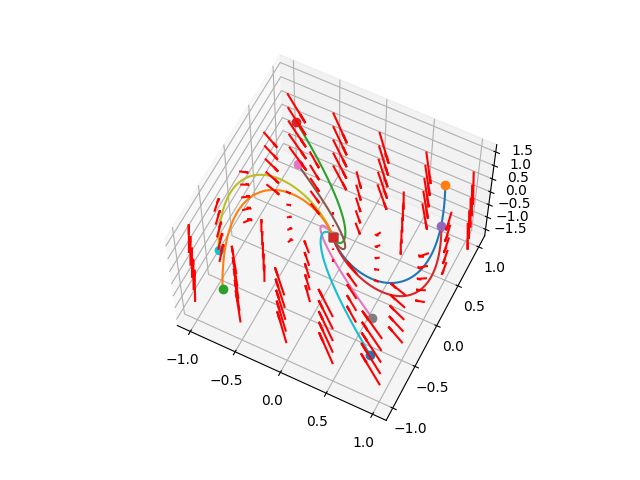
\includegraphics[width=400px]{Figure_1.png}}
\end{DoxyImageNoCaption}
  
\begin{DoxyImageNoCaption}
  \mbox{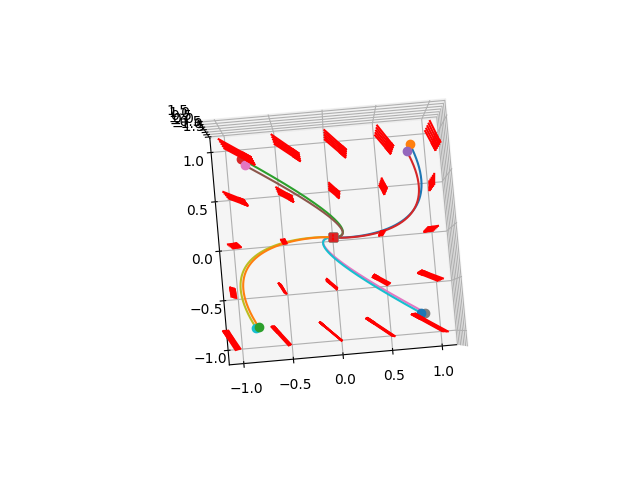
\includegraphics[width=400px]{Figure_2.png}}
\end{DoxyImageNoCaption}
  
\begin{DoxyImageNoCaption}
  \mbox{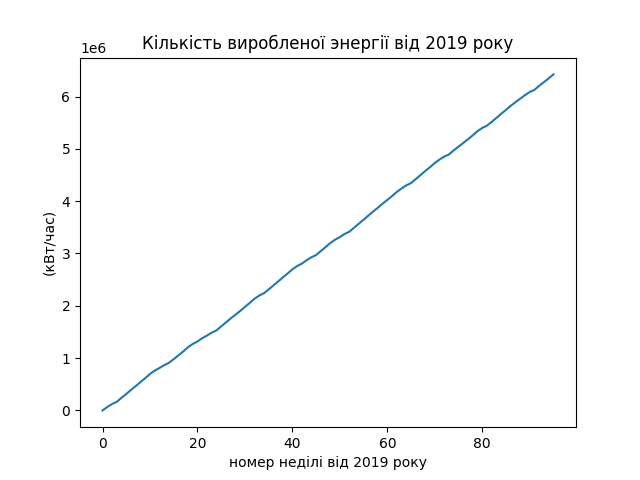
\includegraphics[width=400px]{Figure_3.png}}
\end{DoxyImageNoCaption}
\hypertarget{index_autotoc_md3}{}\doxysubsubsection{Лабораторна робота 2}\label{index_autotoc_md3}
 
\begin{DoxyImageNoCaption}
  \mbox{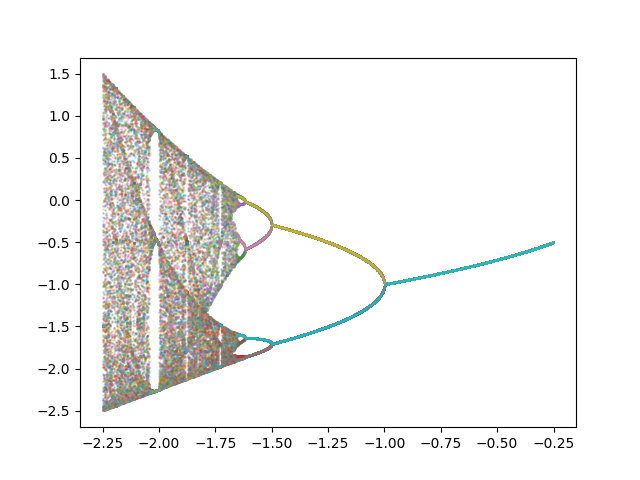
\includegraphics[width=400px]{Figure_2_1.png}}
\end{DoxyImageNoCaption}
  
\begin{DoxyImageNoCaption}
  \mbox{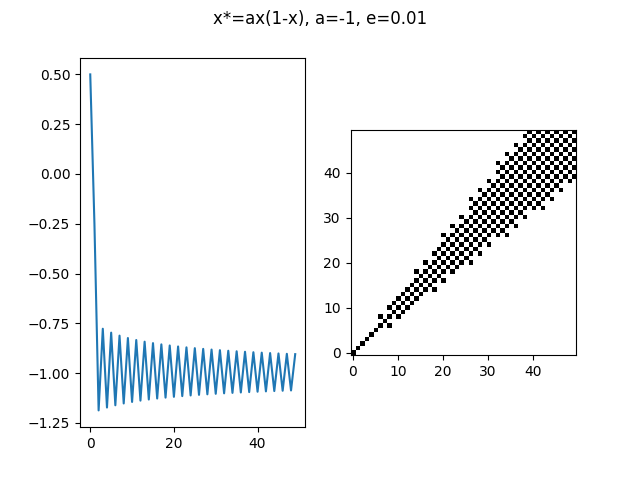
\includegraphics[width=400px]{Figure_2_2.png}}
\end{DoxyImageNoCaption}
  
\begin{DoxyImageNoCaption}
  \mbox{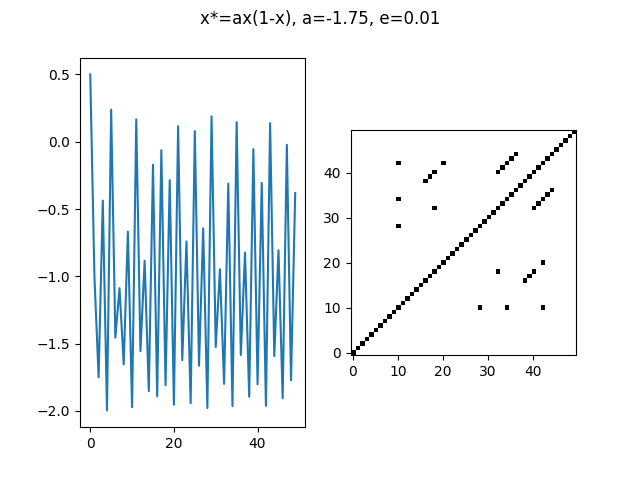
\includegraphics[width=400px]{Figure_2_3.png}}
\end{DoxyImageNoCaption}
  
\begin{DoxyImageNoCaption}
  \mbox{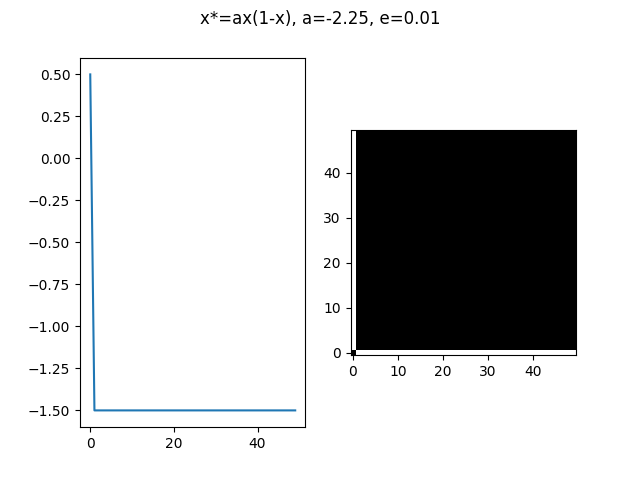
\includegraphics[width=400px]{Figure_2_4.png}}
\end{DoxyImageNoCaption}
\hypertarget{index_autotoc_md4}{}\doxysubsubsection{Лабораторна робота 3}\label{index_autotoc_md4}
 
\begin{DoxyImageNoCaption}
  \mbox{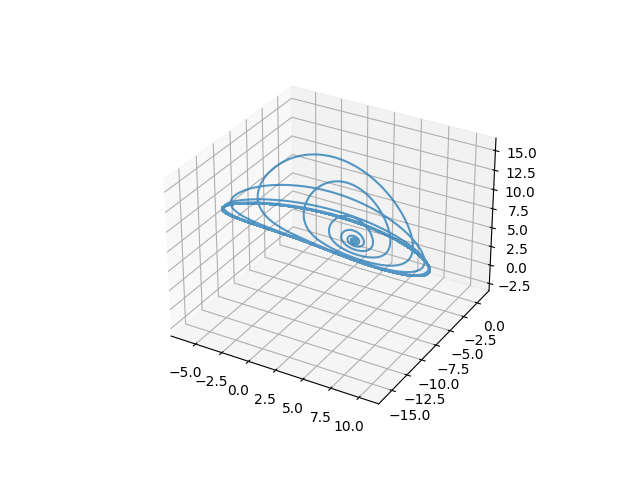
\includegraphics[width=400px]{Figure_3_1.png}}
\end{DoxyImageNoCaption}
  
\begin{DoxyImageNoCaption}
  \mbox{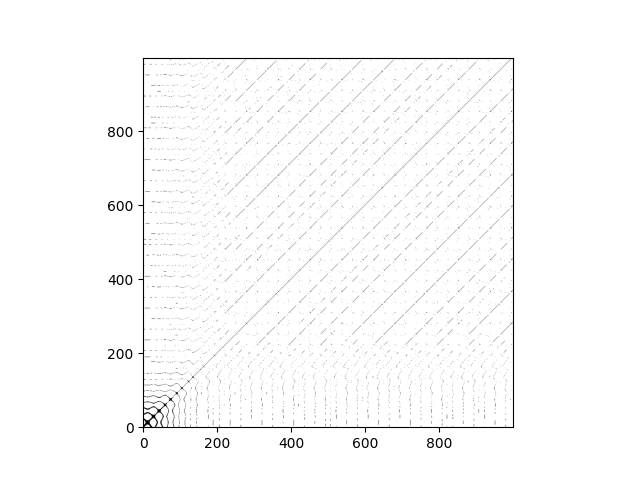
\includegraphics[width=400px]{Figure_3_2.png}}
\end{DoxyImageNoCaption}
  
\begin{DoxyImageNoCaption}
  \mbox{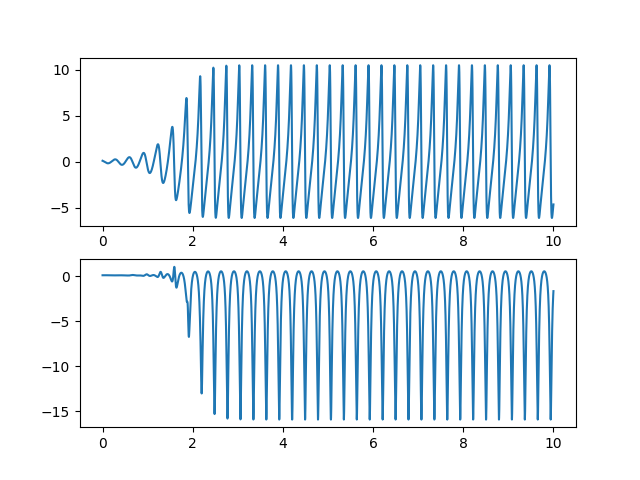
\includegraphics[width=400px]{Figure_3_3.png}}
\end{DoxyImageNoCaption}
  
\begin{DoxyImageNoCaption}
  \mbox{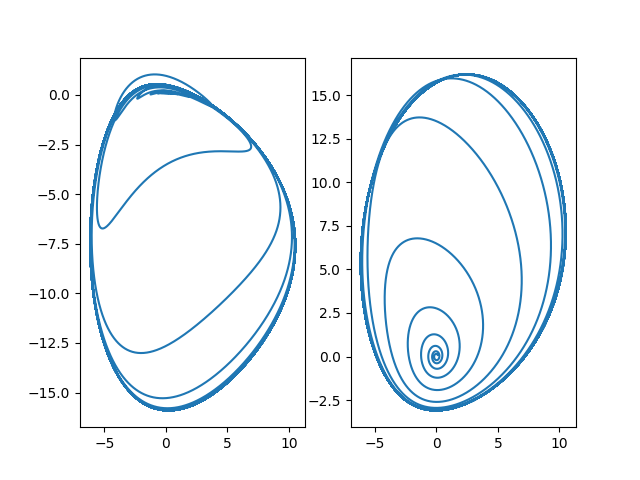
\includegraphics[width=400px]{Figure_3_4.png}}
\end{DoxyImageNoCaption}
  
\begin{DoxyImageNoCaption}
  \mbox{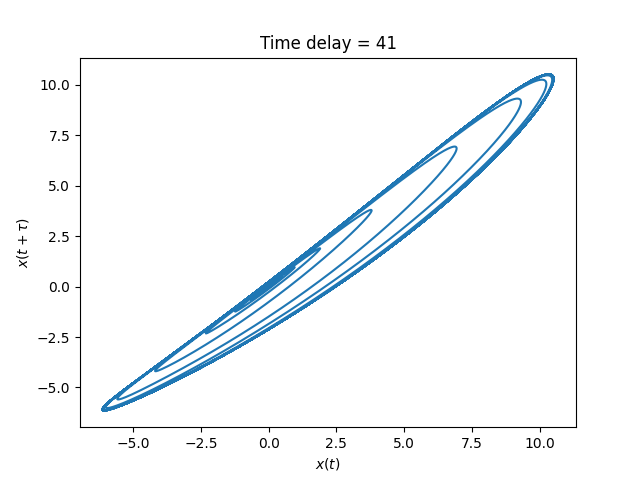
\includegraphics[width=400px]{Figure_3_5.png}}
\end{DoxyImageNoCaption}
  
\begin{DoxyImageNoCaption}
  \mbox{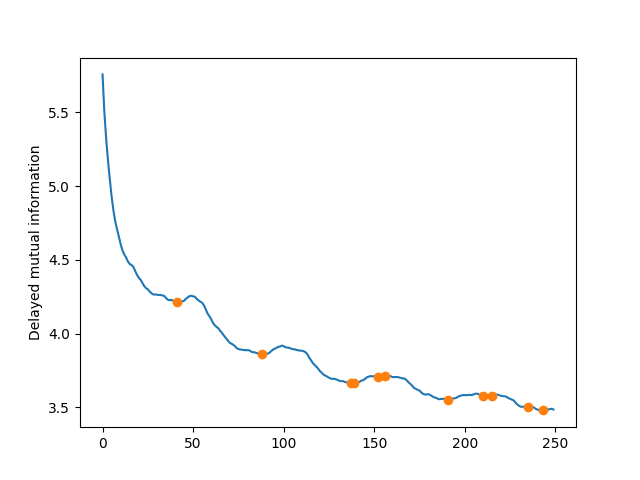
\includegraphics[width=400px]{Figure_3_6.png}}
\end{DoxyImageNoCaption}
  
\begin{DoxyImageNoCaption}
  \mbox{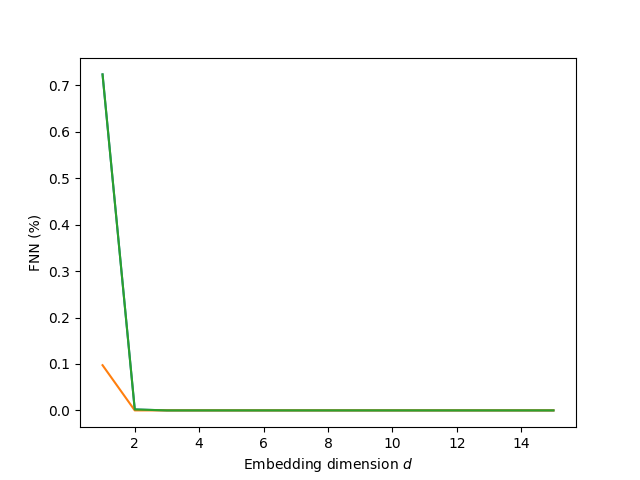
\includegraphics[width=400px]{Figure_3_7.png}}
\end{DoxyImageNoCaption}
  
\begin{DoxyImageNoCaption}
  \mbox{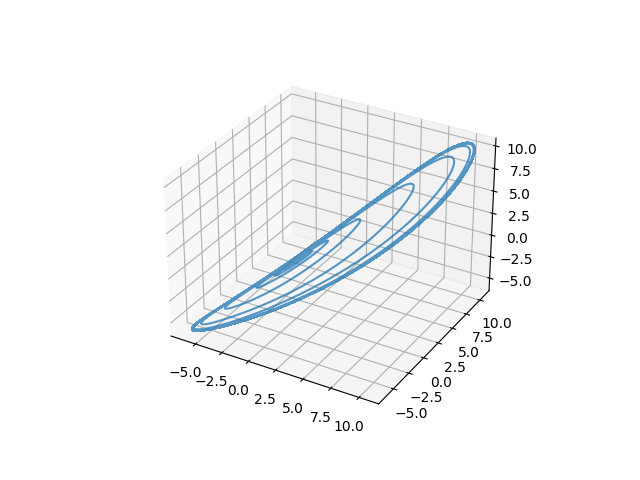
\includegraphics[width=400px]{Figure_3_8.png}}
\end{DoxyImageNoCaption}
 
%--- End generated contents ---

% Index
\newpage
\phantomsection
\clearemptydoublepage
\addcontentsline{toc}{section}{Предметний покажчик}
\printindex

\end{document}
